\documentclass[11pt]{article}
%Gummi|065|=)

\usepackage{amsmath}
\usepackage{amsfonts}
\usepackage{amssymb}
\usepackage{graphicx}

\title{\textbf{Trix: Arrays in 3D}}
\author{Fernando Pujaico Rivera}
\date{}
\begin{document}

\maketitle

\section{Trix}
\subsection{Definition}

A trix $\mathbf{A}\in \mathbb{R}^{M\times N\times L}$ is an array in $3D$, with elements $a_{mnl}$, 
$\{m,n,l\}\in\mathbb{N}$, $1 \leq m \leq M$, $1 \leq n \leq N$, $1 \leq l \leq L$.
\subsection{Examples}
 
The Fig. \ref{fig:trix1} represents a trix $\mathbf{A}\in \mathbb{R}^{4\times 3\times 2}$.
\begin{figure}[h]
  \caption{Trix A}
  \centering
    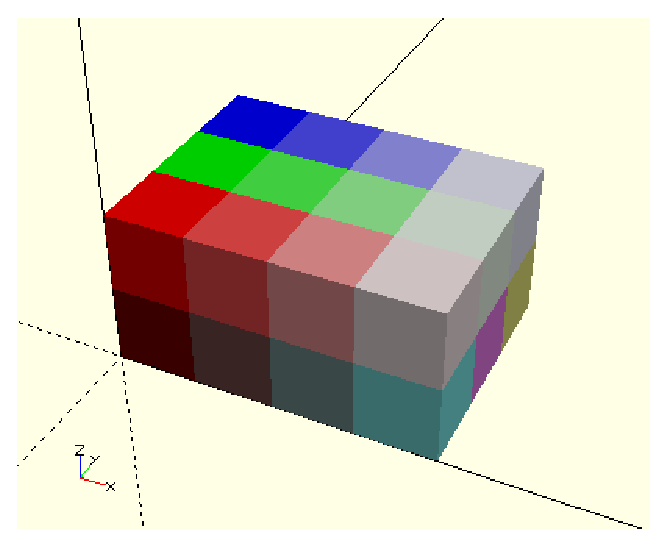
\includegraphics[width=0.5\textwidth]{array3d}
    \label{fig:trix1}
\end{figure}

\end{document}
